\documentclass{article}
\usepackage{graphicx} % Required for inserting images
\usepackage{graphicx} % Required for inserting images
%\usepackage[left=0.5in, right=0.5in, top=0.5in, bottom=0.5in]{geometry}
%\usepackage[left=1.5cm, right=1cm, top=0.5cm, bottom=1.5cm]{geometry}
\usepackage[left=1.5cm, right=1.5cm, top=0.5cm, bottom=1.5cm]{geometry}
\usepackage{amsmath}
\usepackage{amssymb}
\usepackage{amsfonts}
\usepackage{amsthm}
\usepackage{ulem}
\usepackage{bm}
\usepackage{tikz}
\usepackage{enumitem}
\usetikzlibrary{shapes,backgrounds}

\date{}

\begin{document}
\fontsize{13}{15} \selectfont %This is 13pt text with 15pt line spacing.

\begin{center}
 \text{Potterhouse School. \hspace{1cm} Year 6 Math - Homework T1 W11 d.} \qquad \\ 
\vspace{5pt}

%Name: ...........................................................  \hspace{0.5cm}  Date: ....................... \hspace{0.5cm}  Class: ......\hspace{0.5cm} \\
\vspace{5pt}
    Copy the questions and provide solutions.   \\
\vspace{5pt}
    
\includegraphics[width=15cm]{Year_6_Mixed_Tests/Xx.png}
\end{center}

\begin{enumerate}

\item \quad Use equivalent fractions to solve: $ \displaystyle \frac{4}{7} + \displaystyle \frac{3}{14} $ 
\vspace{8pt}

\item \quad Multiply the numerator by the numerator and the denominator by the denominator. 
Then simplify (where needed).
\( \displaystyle \frac{5}{6} \times \displaystyle \frac{13}{9} \) 
\vspace{8pt}

\item \quad Multiply by the reciprocal of 4. 

\( \displaystyle \frac{3}{5} \div \text{\Large 4} \) 
\vspace{8pt}

\item \quad Use the LCM method to solve: \( \displaystyle\frac{2}{3} + \displaystyle \frac{4}{5} \) 
\vspace{8pt}

\item \quad Work out: \( \displaystyle \frac{3}{4} \text{ of } \large 36 \)  
\vspace{8pt}

\item \quad Order the fractions from the smallest to the largest. 

\( \displaystyle \frac{2}{3} \hspace{1cm} \displaystyle \frac{4}{5} \hspace{1cm} \displaystyle \frac{3}{4}  \hspace{1cm} \displaystyle \frac{5}{6}  \vspace{8pt} \)

\item \quad Make the fractions equivalent by multipying both the numerator and the denominator with the same number. 

\( \displaystyle \frac{2}{7} =  \genfrac{}{}{1pt}{0}{\fbox{\makebox[1em]{\rule{0pt}{1em}}}}{28} \)
\vspace{5pt}

\item \quad Sort these numbers into the Venn diagram below. Remember, numbers that fit in both circles to be put at the point of intersection (the central oval). Numbers that do not belong to any circle should be put in the sample space (between the rectangle and the circles). 
\[ 2, 3, 4, 5, 7, 9, 10, 11, 12, 13, 14, 15 \]
\begin{center}
 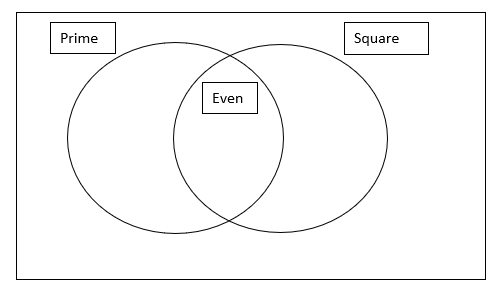
\includegraphics[width=10cm]{Year_6_Mixed_Tests/Homework_Tasks/Venn1.png}   
\end{center}
 
\end{enumerate}




\end{document}